\documentclass[12pt, letterpaper]{article}
\usepackage[english]{babel}
\usepackage{graphicx}
\usepackage{framed}
\usepackage[normalem]{ulem}
\usepackage{amsmath}
\usepackage{amsthm}
\usepackage{amssymb}
\usepackage{amsfonts}
\usepackage{enumerate}
\usepackage{listings}
\usepackage[utf8]{inputenc}
\usepackage[top=1 in,bottom=1in, left=1 in, right=1 in]{geometry}
\usepackage{tikz}


%bunch of definitions
\newcommand{\R}{\mathbb{R}}
\newcommand{\N}{\mathbb{N}}
\newcommand{\Q}{\mathbb{Q}}
\newcommand{\Z}{\mathbb{Z}}
\def\trans{^\mathrm{T}}
\theoremstyle{definition}
\newtheorem{theorem}{Theorem}
\newtheorem{corollary}{Corollary}
\newtheorem*{definition}{Definition}
\newtheorem*{example}{Example}
\newtheorem*{note}{Note}
\newtheorem{exercise}{Exercise}
\newcommand{\bproof}{\bigskip {\bf Proof. }}
\newcommand{\eproof}{\hfill\qedsymbol}
\newcommand{\Disp}{\displaystyle}
\newcommand{\qe}{\hfill\(\bigtriangledown\)}
\setlength{\columnseprule}{1 pt}

% Setlength w/ parskip includes space after headers as well
% \setlength{\parskip}{4mm}
\setlength{\parindent}{0mm}
% No space after headers; but a bit larger spacing between words
\usepackage[parfill]{parskip}

%====================================
%====== To highlight single matrix element ===
%====================================
\usepackage{xcolor}% http://ctan.org/pkg/xcolor
\newcommand{\highlight}[1]{%
  \ooalign{\hss\makebox[0pt]{\fcolorbox{gray!90}{white}{$#1$}}\hss\cr\phantom{$#1$}}%
}
%==============

\newcommand{\beginmatrix}[1]{%
    \left[ \begin{array}{#1}
}
\renewcommand{\endmatrix}{\end{array} \right]}

% Defining styling for code snippets
\definecolor{codegreen}{rgb}{0,0.6,0}
\definecolor{codegray}{rgb}{0.5,0.5,0.5}
\definecolor{codepurple}{rgb}{0.58,0,0.82}
\definecolor{backcolour}{rgb}{0.95,0.95,0.92}

\lstdefinestyle{mystyle}{
    backgroundcolor=\color{backcolour},   
    commentstyle=\color{codegreen},
    keywordstyle=\color{magenta},
    numberstyle=\tiny\color{codegray},
    stringstyle=\color{codepurple},
    basicstyle=\ttfamily\footnotesize,
    breakatwhitespace=false,         
    breaklines=true,                 
    captionpos=b,                    
    keepspaces=true,                 
    numbers=left,                    
    numbersep=5pt,                  
    showspaces=false,                
    showstringspaces=false,
    showtabs=false,                  
    tabsize=2
}
\lstset{style=mystyle}


\begin{document}

\section*{Misc Things}

\begin{center}
  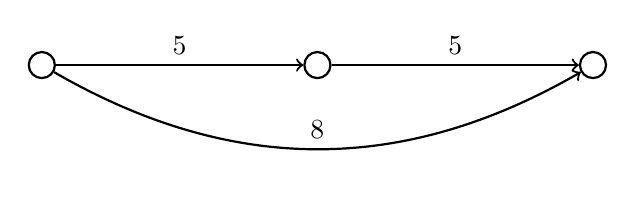
\begin{tikzpicture} [node distance={35mm}, thick, main/.style = {draw, circle}]
    \node[main] (1) {};
    \node[main] (2)[right of=1] {};
    \node[main] (3)[right of=2] {};

    \draw[->](1) edge node[above, sloped] {5} (2);
    \draw[->](2) edge node[above, sloped] {5} (3);
    \draw[->](1) edge[bend right] node[above, sloped] {8} (3);

  \end{tikzpicture}
\end{center}

\begin{lstlisting}[language=Python, mathescape=true]
  def functionThing(A, C):
      maxVal = $max_{1 \leq i \leq n} v_i$
      for i from 1 to n:
          for j from 0 to W:
              for k from 0 to maxVal:
                  do stuff
      return thing
  \end{lstlisting}

% Big Bracket thing
\[
    V[i,j,k] = 
    \begin{cases} 
      0 & i = 0 \text{ or } j = 0 \\
      Two & \text{if } 2  \\
      three &  3
   \end{cases}
\]



\end{document}


% MATRIX SAMPLE

% \begin{align*}
%     &  % the ampersand indicates the location of the alignment
%     \beginmatrix{cc|c}
%     1 & 2 & a \\
%     5 & \highlight{6} & 10
%     \endmatrix
%     \\  % new line
%     &
%     \begin{array}{c}
%     \\
%     (2) + \frac{1}{2} (1)
%     \end{array}
%     \beginmatrix{cc|c}
%     x & y & z \\
%     a & b & c
%     \endmatrix
% \end{align*}